%! Tex program = xelatex   
\documentclass{article}
\usepackage{graphicx,subfig}
\usepackage[left=2cm, right=2cm, lines=45, top=0.8in, bottom=0.7in]{geometry}
\usepackage{xeCJK}
\usepackage{amsmath}
\usepackage{booktabs} %表格
\usepackage{tikz}
\usepackage{graphics}
\usepackage{xcolor} 
\usepackage{tikz} 
\usepackage{svg}
\usetikzlibrary{arrows,shapes,chains}
\setmainfont{Times New Roman}
\setCJKmainfont{Songti SC}
\setCJKfamilyfont{song}{Songti SC}
\renewcommand{\baselinestretch}{1.5} %行间距
%-----------------------伪代码------------------
\usepackage{algorithm}  
\usepackage{algorithmicx}  
\usepackage{algpseudocode}  
\floatname{algorithm}{Algorithm}  
\renewcommand{\algorithmicrequire}{\textbf{Input:}}  
\renewcommand{\algorithmicensure}{\textbf{Output:}} 
\usepackage{lipsum}  
\makeatletter
\newenvironment{breakablealgorithm}
  {% \begin{breakablealgorithm}
  \begin{center}
     \refstepcounter{algorithm}% New algorithm
     \hrule height.8pt depth0pt \kern2pt% \@fs@pre for \@fs@ruled
     \renewcommand{\caption}[2][\relax]{% Make a new \caption
      {\raggedright\textbf{\ALG@name~\thealgorithm} ##2\par}%
      \ifx\relax##1\relax % #1 is \relax
         \addcontentsline{loa}{algorithm}{\protect\numberline{\thealgorithm}##2}%
      \else % #1 is not \relax
         \addcontentsline{loa}{algorithm}{\protect\numberline{\thealgorithm}##1}%
      \fi
      \kern2pt\hrule\kern2pt
     }
  }{% \end{breakablealgorithm}
     \kern2pt\hrule\relax% \@fs@post for \@fs@ruled
  \end{center}
  }
\makeatother
%------------------------代码-------------------
\usepackage{xcolor} 
\usepackage{listings} 
\usepackage{fontspec}
\newfontfamily\menlo{Menlo}
\setmonofont[Mapping={}]{Monaco} 
\definecolor{mygreen}{rgb}{0,0.6,0}
\definecolor{mygray}{rgb}{0.5,0.5,0.5}
\definecolor{mymauve}{rgb}{0.58,0,0.82}
\lstset{ %
backgroundcolor=\color{white},   % choose the background color
basicstyle=\footnotesize\ttfamily,        % size of fonts used for the code
columns=fullflexible,
breaklines=true,                 % automatic line breaking only at whitespace
captionpos=b,                    % sets the caption-position to bottom
tabsize=4,
commentstyle=\color{mygreen},    % comment style
escapeinside={\%*}{*)},          % if you want to add LaTeX within your code
keywordstyle=\color{blue},       % keyword style
stringstyle=\color{mymauve}\ttfamily,     % string literal style
frame=single,
rulesepcolor=\color{red!20!green!20!blue!20},
numbers=left,
 numberstyle=\tiny\menlo
% identifierstyle=\color{red},
% language=c++,
}
\begin{document}
\title{RNN实验报告}
\author{朱浩泽 1911530}
\maketitle
\large
\section{老师提供的原始版本RNN网络结构}
\subsection{网络结构}
\begin{lstlisting}
RNN(
  (i2h): Linear(in_features=185, out_features=128, bias=True)
  (i2o): Linear(in_features=185, out_features=18, bias=True)
  (softmax): LogSoftmax(dim=1)
)
\end{lstlisting}
\subsection{实验结果}
\begin{figure}[H]
   \centering
   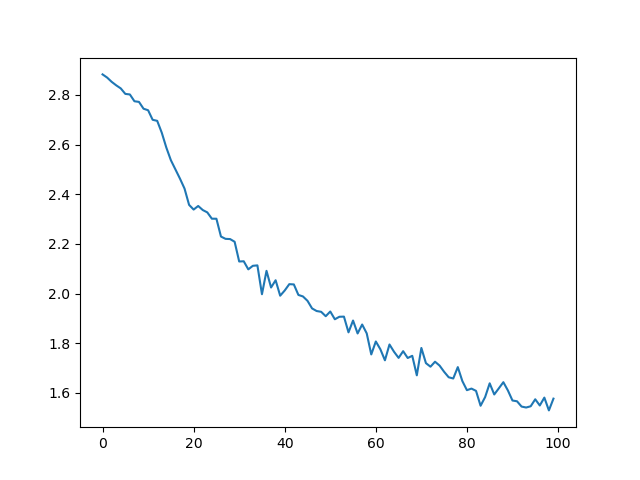
\includegraphics[scale= 0.5]{validation_loss.png}
   \caption{\textbf{RNN的损失}}
\end{figure}
\begin{figure}[H]
   \centering
   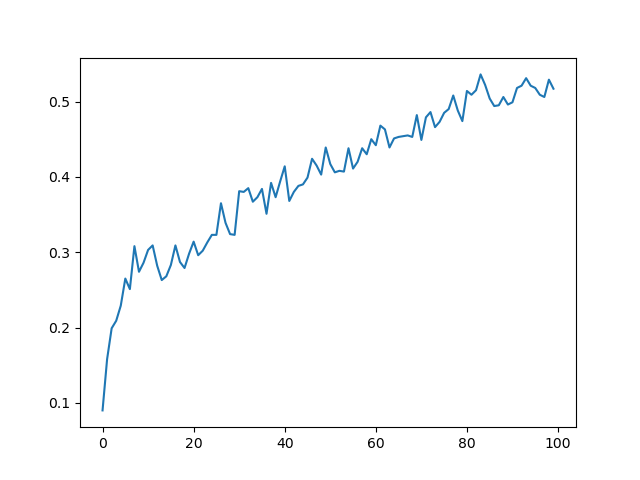
\includegraphics[scale= 0.5]{validation_accuracy.png}
   \caption{\textbf{RNN的准确率}}
\end{figure}
\begin{figure}[H]
   \centering
   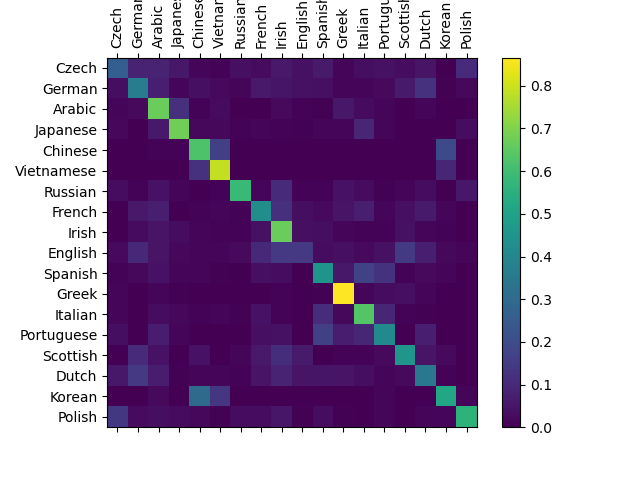
\includegraphics[scale= 0.5]{1.png}
   \caption{\textbf{RNN的预测准确图}}
\end{figure}

\section{利用Pytorch搭建的LSTM}
\subsection{网络结构}
\begin{lstlisting}
LSTM(
  (lstm): LSTM(57, 128, num_layers=2)
  (linear): Linear(in_features=128, out_features=18, bias=True)
  (softmax): LogSoftmax(dim=1)
)
\end{lstlisting}
\subsection{实验结果}
\begin{figure}[H]
   \centering
   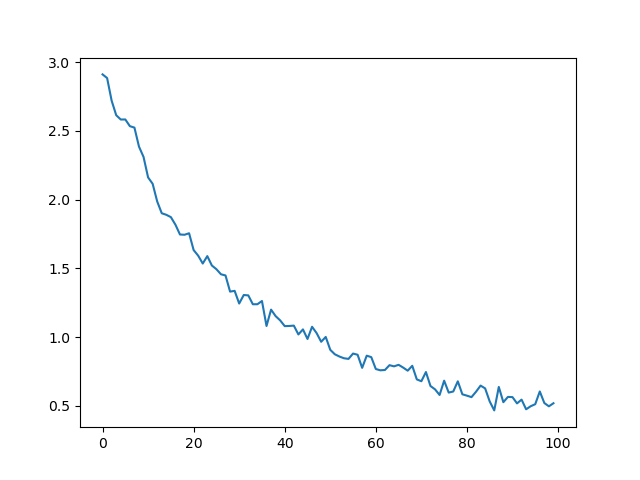
\includegraphics[scale= 0.5]{LSTM_.png}
   \caption{\textbf{LSTM的损失}}
\end{figure}
\begin{figure}[H]
   \centering
   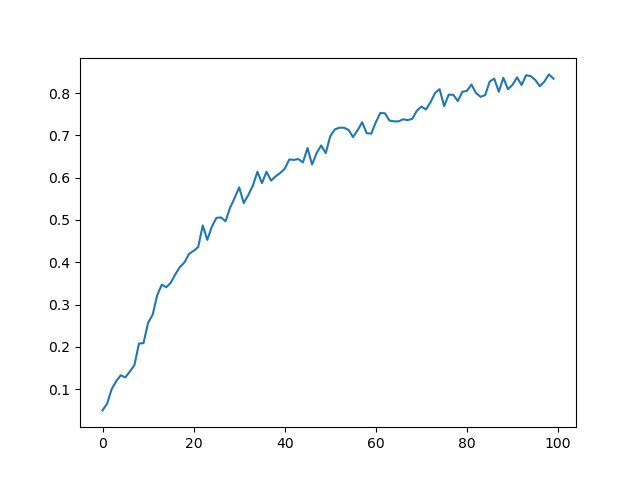
\includegraphics[scale= 0.5]{LSTM_validation_accuracy.png}
   \caption{\textbf{LSTM的准确率}}
\end{figure}
\begin{figure}[H]
   \centering
   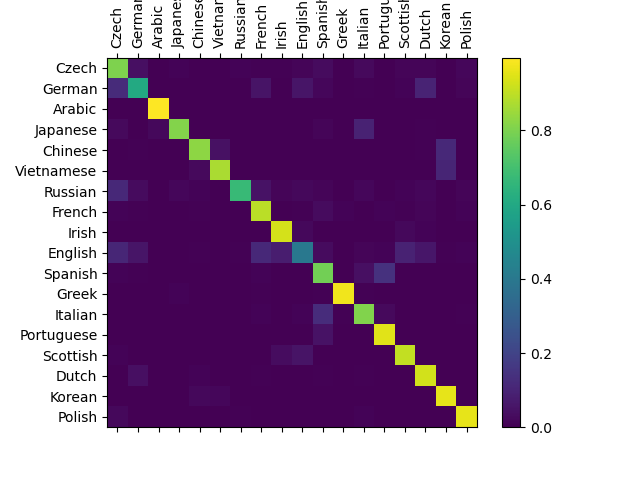
\includegraphics[scale= 0.5]{2.png}
   \caption{\textbf{LSTM的预测准确图}}
\end{figure}
\section{为什么LSTM网络的性能优于RNN网络}
RNN即循环神经网络,其可以处理一定的短期依赖,但是对长序列进行学习时,循环神经网络会出现梯度消失和梯度爆炸现象,无法掌握长时间跨度的非线性关系。这种现象的主要原因是,当序列比较长的时候,序列后部的梯度很难反向传播到前面的序列,这便导致了前面提到的问题。假设$h_t$指的是时间t时刻的隐藏层状态值,$x_t$为t时刻的输入,我们可以通过以下公式进行进行隐藏层的计算
$$
h_t = tanh(W_t\cdot [h_t, x_t] + b_h)
$$
可以看出,传统的RNN的任意时刻的隐藏层获取的信息只来源于当前输入和上一时刻的隐藏层的信息,没有任何记忆功能,所以并不能处理长程依赖。


而1997年Long Short Memory一种提出的LSTM结构,巧妙的应用了自循环的思想产生了梯度长时间持续流动的路径来解决了这一问题。具体来说,LSTM网络引入了三个门控机制来控制信息传递的路径,分别是输入门$i_t$、遗忘门$f_t$和输出门$o_t$。
\begin{itemize}
   \item 遗忘门 $f_t$ 控制上一个时刻的内部状态 $c_{t−1}$ 需要遗忘多少信息
   \item 输入门 $i_t$  控制当前时刻的候选状态 $\tilde{c_t}$  有多少信息需要保存
   \item  输出门 $o_t$ 控制当前时刻的内部状态 $c_t$ 有多少信息需要输出给外部状态$h_t$
\end{itemize}
其具体的计算公式为
\begin{align*}
   i_t &= \sigma(W_ix_t + U_ih_{t-1} + b_i)\\
   f_t &= \sigma(W_fx_f + U_fh_{t-1} + b_f)\\
   o_t &= \sigma(W_ox_o + U_oh_{t-1} + b_0)\\
\end{align*}
具体计算过程为首先利用上一 时刻的外部状态 $h_{t-1}$ 和当前时刻的输入$x_t$,计算出三个门,以及候选状态$\tilde{c_t}$,结合遗忘门 $f_t$ 和输入门 $i_t$ 来更新记忆单元 $c_t$,结合输出门$o_t$,将内部状态的信息传递给外部状态 $h_t$。
和RNN的隐状态$h$相同,LSTM中的隐藏层也存储了历史信息。在基础的RNN中,隐状态每个时刻都会被重写,因此可以看作一种短期记忆。而长期记忆则可以看作是一种网络参数,隐含了从训练数据中学到的经验,其更新周期要远远慢于RNN的隐藏层的更新。而在LSTM网络中,记忆单元 $c$ 可以在某个时刻捕捉到某个关键信息,并有能力将此关键信息保存一定的时间间隔。记忆单元 $c$ 中保存信息的生命周期要长于短期记忆$h$,所以LSTM可以更好的学习到长程依赖。而文字中有时需要利用上下文信息才可以更好的进行理解,所以LSTM网络的性能优于RNN。

\end{document}
